\begin{figure*}[t]
	\centering
	\begin{subfigure}{0.33\linewidth}
		{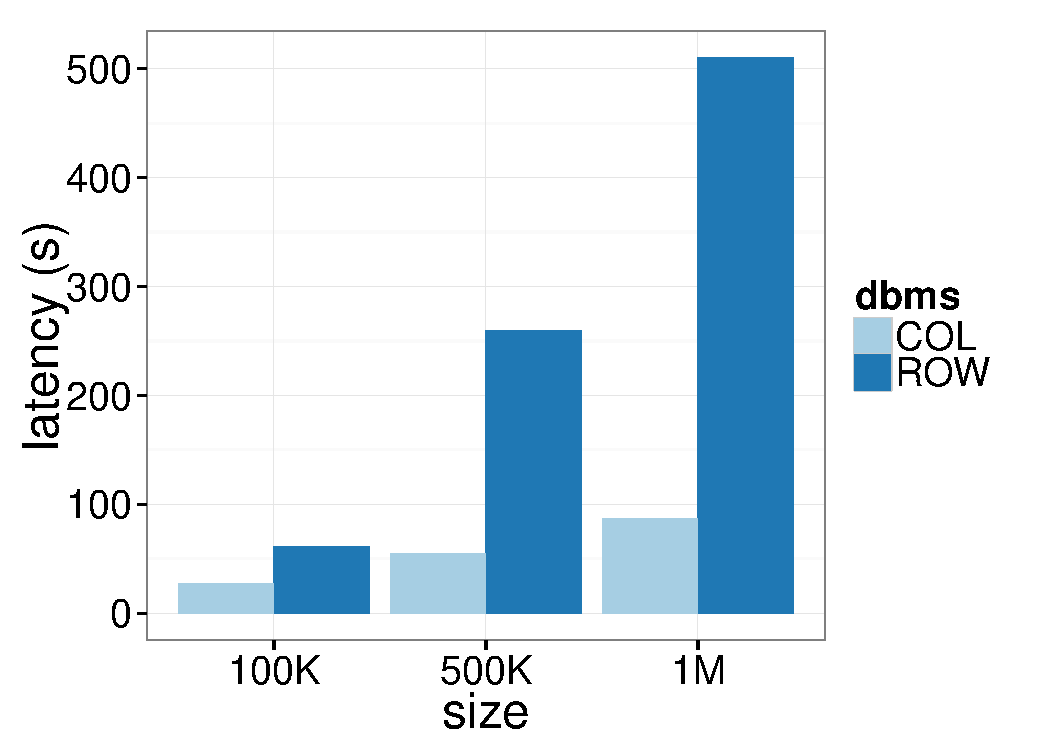
\includegraphics[width=6cm] {Images/baselines_by_size.pdf}}
		\caption{Latency vs. Table size}
		\label{fig:baseline_size}
	\end{subfigure}
	\begin{subfigure}{0.33\linewidth}
		\centering
		{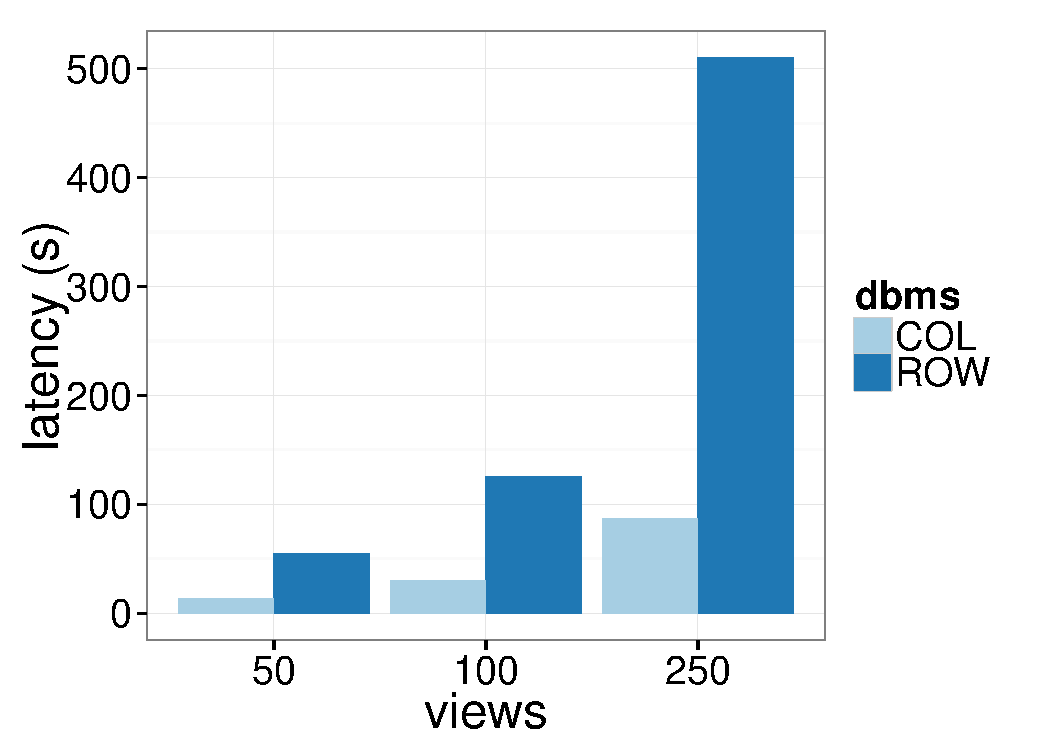
\includegraphics[width=6cm] {Images/baselines_by_views.pdf}}
		\caption{Latency vs. Num Views}
		\label{fig:baseline_views}
	\end{subfigure}
	\begin{subfigure}{0.33\linewidth}
		{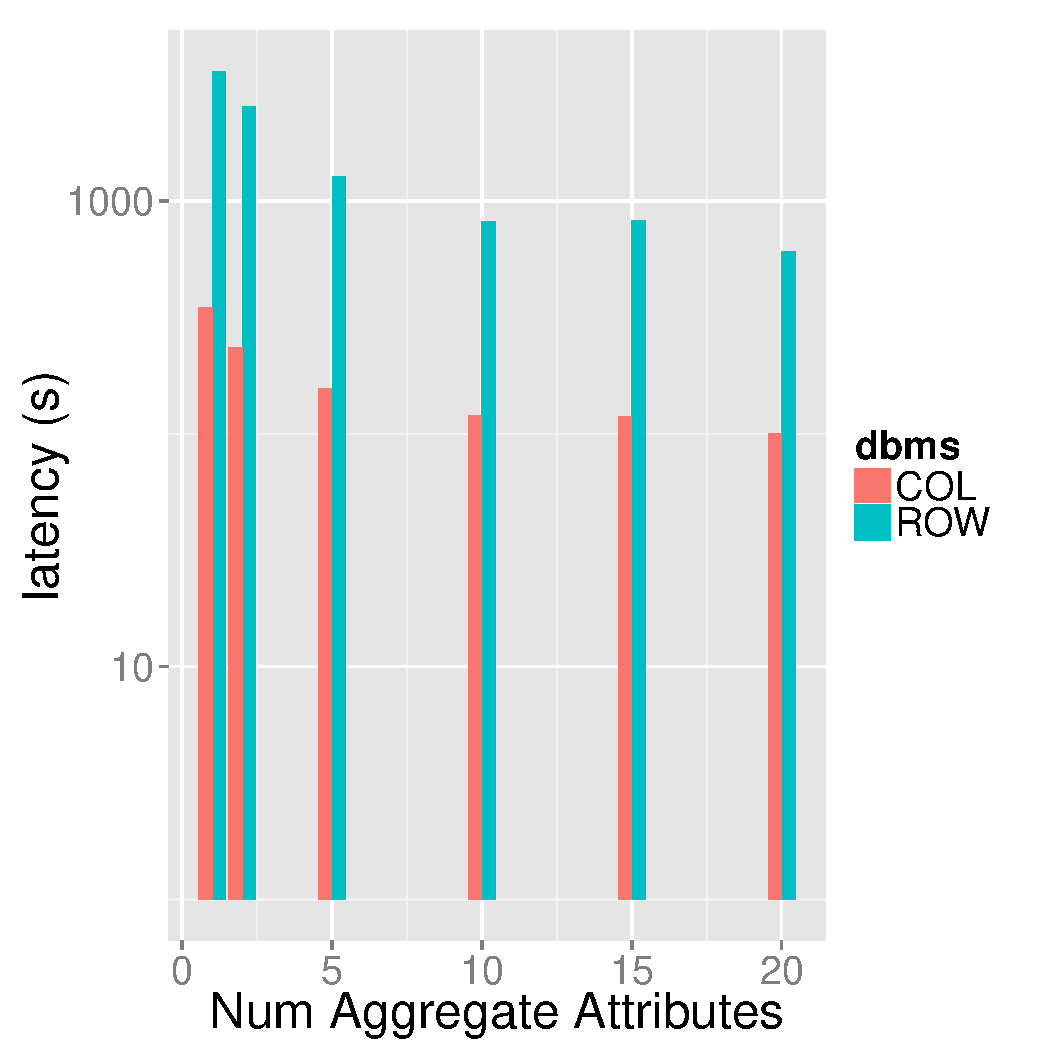
\includegraphics[width=6cm] {Images/multi_agg.pdf}}
		\caption{Latency vs. number of aggregates}
		\label{fig:multi_agg}
	\end{subfigure}
	\vspace{-10pt}
	\caption{Baseline performance and Effect of Combining Aggregates }
	\vspace{-10pt}
	\label{fig:bank_perf}
\end{figure*}

\begin{figure*}[t]
	\centering
	\begin{subfigure}{0.33\linewidth}
		\centering
		{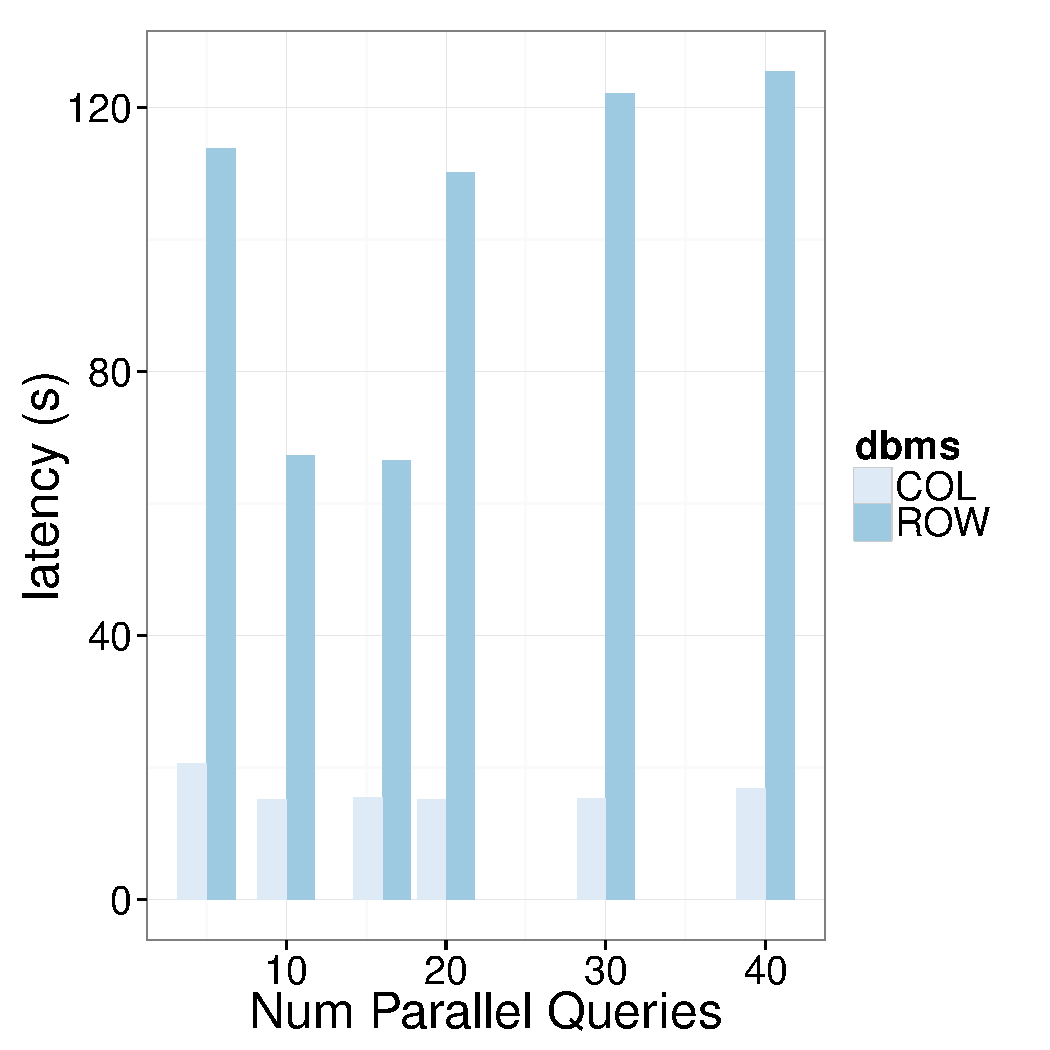
\includegraphics[width=6cm] {Images/parallel_noop.pdf}}
		\caption{Effect of parallelism}
		\label{fig:parallelism}
	\end{subfigure}
	\begin{subfigure}{0.33\linewidth}
		\centering
		{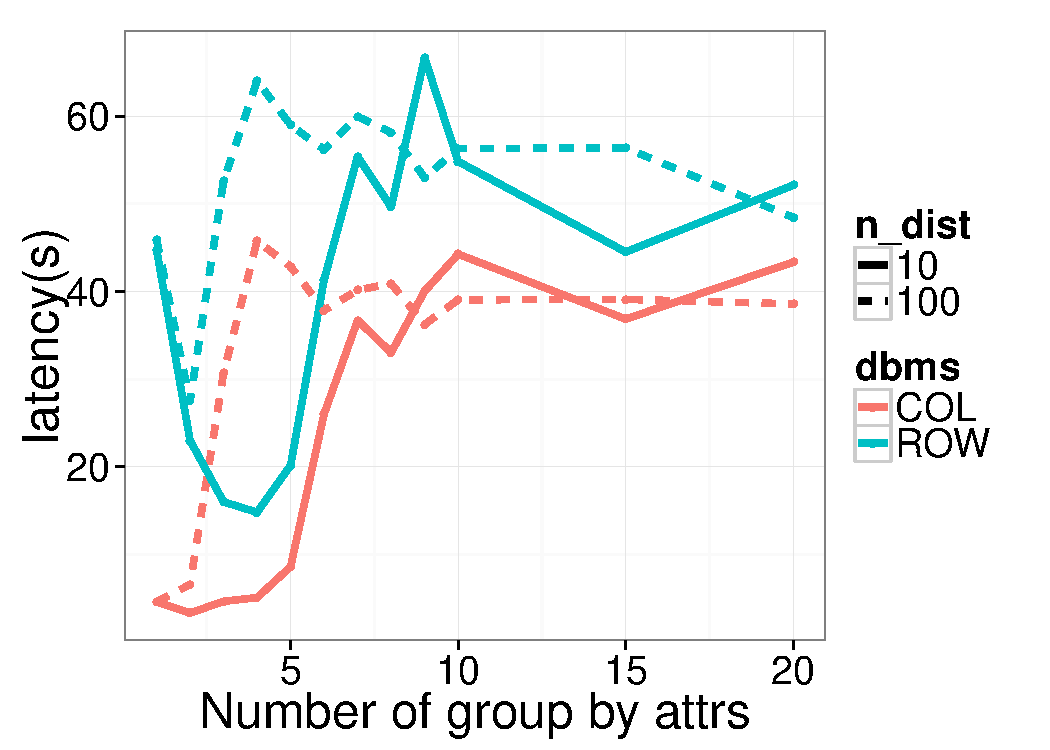
\includegraphics[width=6cm] {Images/multi_gb_same.pdf}}
		\caption{Latency vs. Num of Groups}
		\label{fig:multi_gb_same}
	\end{subfigure}
	\begin{subfigure}{0.33\linewidth}
		\centering
		{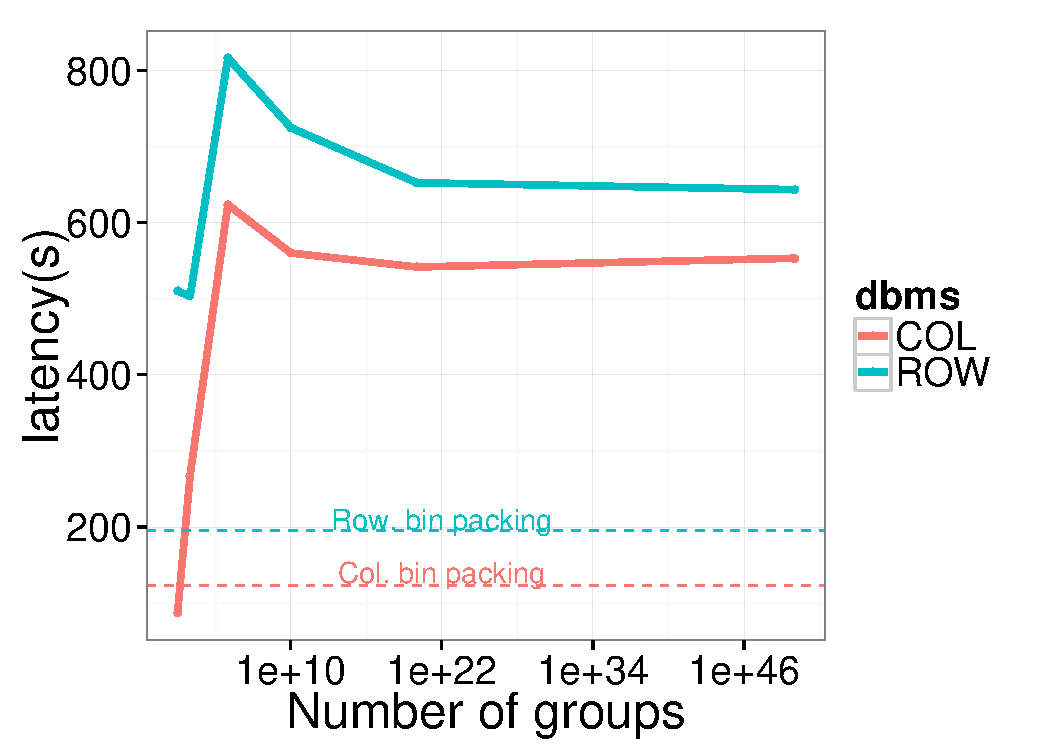
\includegraphics[width=6cm] {Images/multi_gb.pdf}}
		\caption{Latency vs. Num Dimensions}
		\label{fig:multi_gb_bp}
	\end{subfigure}
	\vspace{-10pt}
su	\caption{Effect of Combining Group-by attributes and Parallel Query Execution}
	\label{fig:bank_perf}
	\vspace{-10pt}
\end{figure*}

\subsection{Basic \large{\SeeDB} Framework}
\label{sec:basic_framework_expts}

{\em \underline{Summary:} Applying no optimizations 
leads to latencies in the 100s of seconds for both ROW and COL;
latency increases linearly in the size of the dataset and  number
of views. 
Column stores are superior to row stores,
with $\frac{1}{5}$th the latency.}
Without any optimizations, the basic \SeeDB execution engine
serially executes individual view queries, two for each possible view.
Figure \ref{fig:baseline_size} shows latency of \SeeDB\ vs. the number of rows (100K rows--1M rows) in the dataset while  
Figure \ref{fig:baseline_views} shows latency as a function 
of the number of views (50--250).
This chart shows results for the SYN dataset obtained by varying the size of the
table and number of attributes (SYN is comparable to the AIR dataset).
% and we created subsets of the dataset with
% varying numbers of rows and views, by varying the number of dimension attributes. 
First, notice that the basic no optimization framework has very 
poor performance: latency for ROW is between 50-500s, 
while it is between 10-100s for COL. 
This is because both ROW and COL run 50 to 250 SQL queries for each \SeeDB query.
These time scales are not practical for interactive applications. 
Second, COL runs about 5X faster than ROW. 
This is expected because individual view queries only select one dimension
attribute and one measure attribute at a time.  
COL can just read these two
columns, whereas ROW must read all columns.
Third, as expected, the latency of the
basic framework is proportional to the number of rows as well as the 
number of views in the table.
Since the latencies for the basic framework are very high for interactive
applications, it is clear that aggressive optimization needs to be employed.

\subsection{Sharing Optimizations}
\label{sec:expts_dbms_execution_engine}

% Our primary metric for evaluating the DBMS-backed
% execution engine is {\em latency},
% i.e., .
% Specifically, we study the impact of the following properties on latency:
% (a) parameters of the dataset including size and number of views.
% (b) the optimizations detailed in Section~\ref{sec:dbms_optimizations}, and
% (c) 
% Our goal is to identify which data layout is a better
% fit for \SeeDB, and study the gains of each optimization
% for row-stores vs.~column stores. 
In this section, we study the performance of the sharing optimizations described in Section \ref{sec:sharing_opt}.
Recall that the goal of these optimizations is to reduce the number of queries run against the DBMS and to share scans as much as possible between queries.
The following experiments report results on the synthetic datasets SYN and SYN* 
(Table~\ref{tab:datasets}).
We chose to test these optimizations on synthetic data since we can control all parameters of the data including size, number of attributes, and data distribution.
(Results on real datasets are shown in Figure \ref{fig:share_prune_row} and \ref{fig:share_prune_col}).
We find that our sharing optimizations can provide upto a 40X speedup for ROW and 10X speedup for COL allowing small and moderate sized datasets to be processed at interactive time scales (< 5s) and reduce latency on large datasets from 
500 seconds (ROW) and 100 seconds (COL) to <10 seconds for COL, and <20 seconds for ROW.


\techreport{
\stitle{Result Highlights:}
\begin{denselist}
\item Our optimizations to the DBMS-based execution engine can reduce
latency on large datasets from 500 seconds (ROW) and 100 seconds (COL)
to <10 seconds for COL, and <20 seconds for ROW.
% This is particularly noteworthy given that
% \SeeDB is running 100s of queries on the DBMS for each \SeeDB query.

\item Latency scales linearly 
with dataset size and number of views.

\item Column stores are superior to row stores 
for our workload. Row stores, however, benefit more from the
proposed optimizations. 
% For instance, row stores benefit
% significantly (with reductions of up to 2.5X on latency) from applying
% bin-packing-based algorithms for aggregation, 
% while column stores are not significantly affected. 

\item Although our optimizations lead to a 8X-20X speedup, the total latency remains in the 10s of seconds.
 % - a number unacceptable in interactive systems.
In addition, each \SeeDB query translates to 50+ SQL queries. 
This {\it query bloat} unnecessarily consumes DBMS resources including memory and CPU.
Consequently, we see the need for a custom solution with  lower latencies and a
smaller resource footprint.
\end{denselist}
}

% As mentioned in Section \ref{sec:dbms_execution_engine}, our DBMS-based
% execution engine leverages the DBMS API to execute view queries directly on the
% database.
% While this approach has the advantages of reusing existing query procesing
% systems and being agnostic to the specific underlying DBMS, its limitations
% include the lack of fine grained control over sharing of table scans and lack of
% ability to prune low-utility views. 

% We start with an evaluation of the basic framework (without any optimizations) 
% and then study the effect of the proposed optimizations (Section~\ref{sec:dbms_optimizations}).
% Our goal is to characterize the effect of each optimization and find the optimal parameter 
% settings for the DBMS execution engine.
% , i.e., 
% how long do row and column stores take if each view is evaluated 
% in sequence, without any optimization. 
% We then study the effect of adding each optimization from Section~\ref{sec:dbms_optimizations} 
% in turn.

 

% \begin{figure}[h] 
% \centerline{
% \resizebox{4cm}{!} {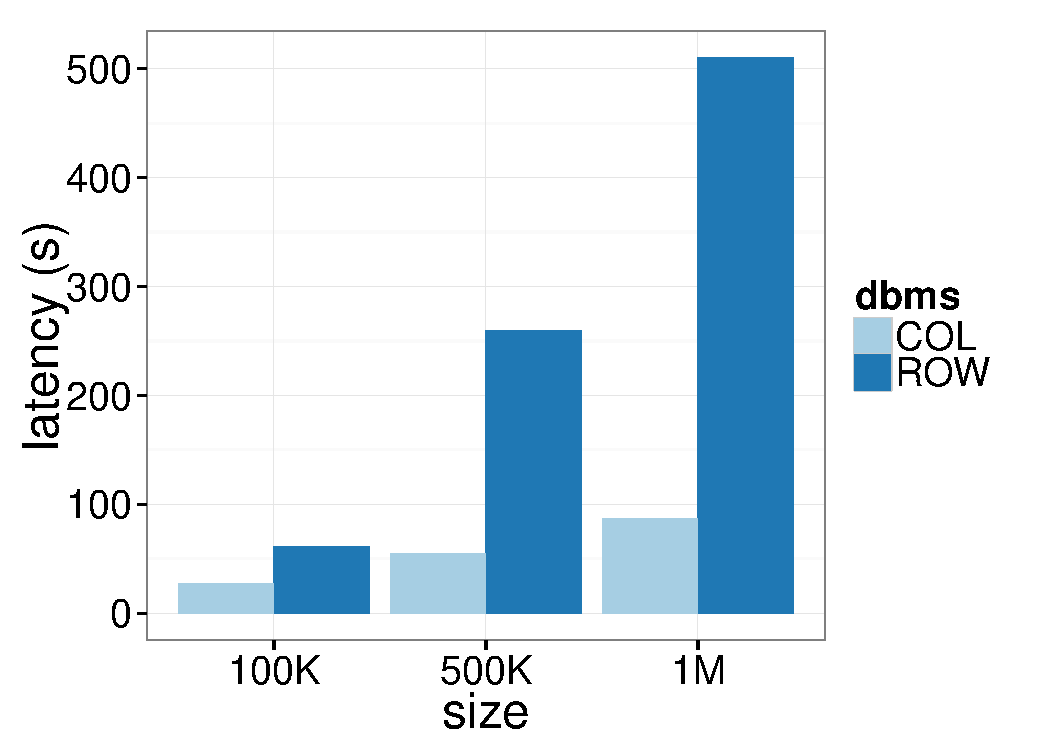
\includegraphics {Images/baselines_by_size.pdf}}
% \resizebox{4cm}{!} {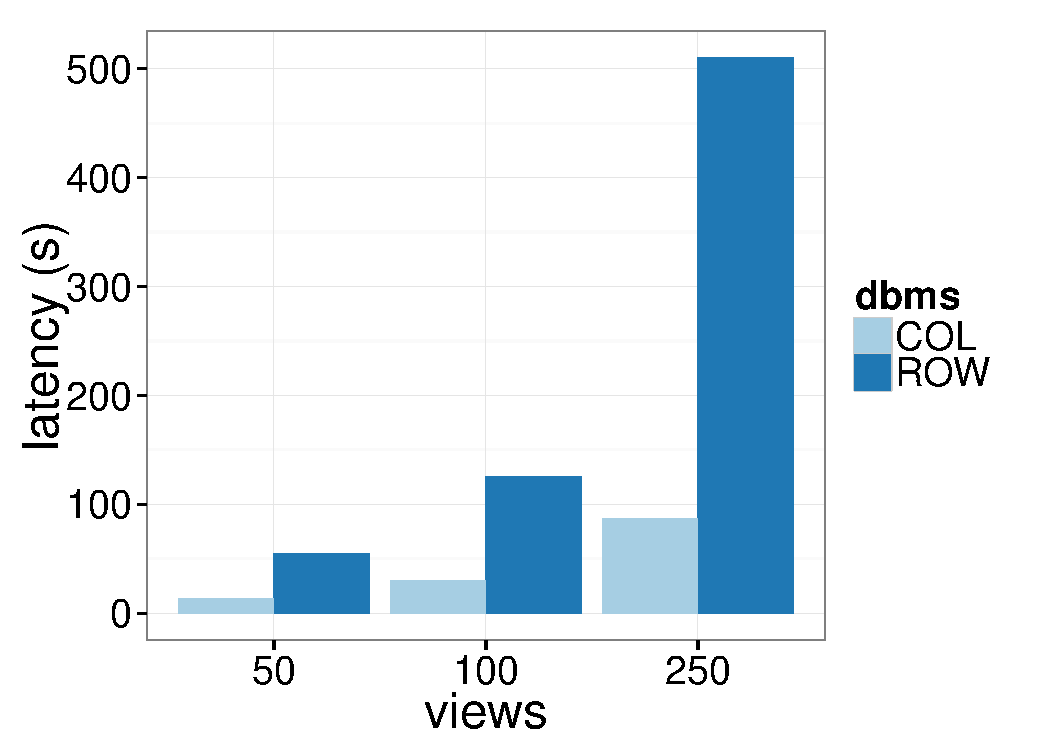
\includegraphics {Images/baselines_by_views.pdf}}
% }
% \end{figure}



% \begin{figure}[h]
% \centering
% \begin{subfigure}{0.49\linewidth}
% \centering
% {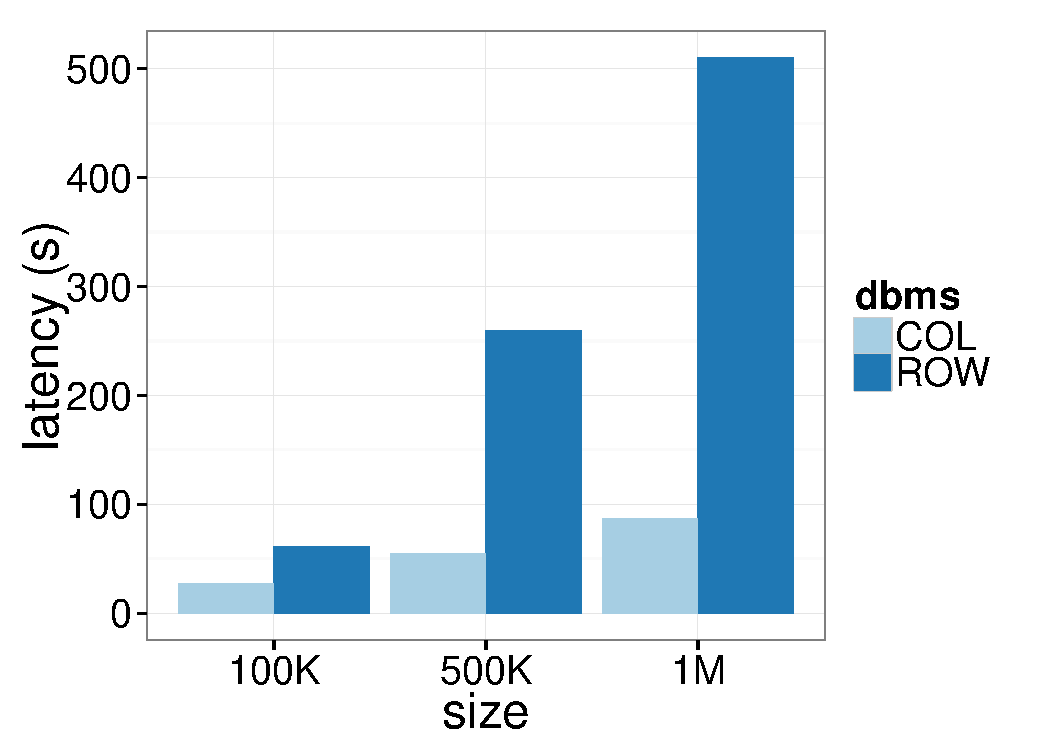
\includegraphics[width=4.2cm] {Images/baselines_by_size.pdf}}
% \caption{Latency vs. Table size}
% \label{fig:baseline_size}
% \end{subfigure}
% \begin{subfigure}{0.49\linewidth}
% \centering
% {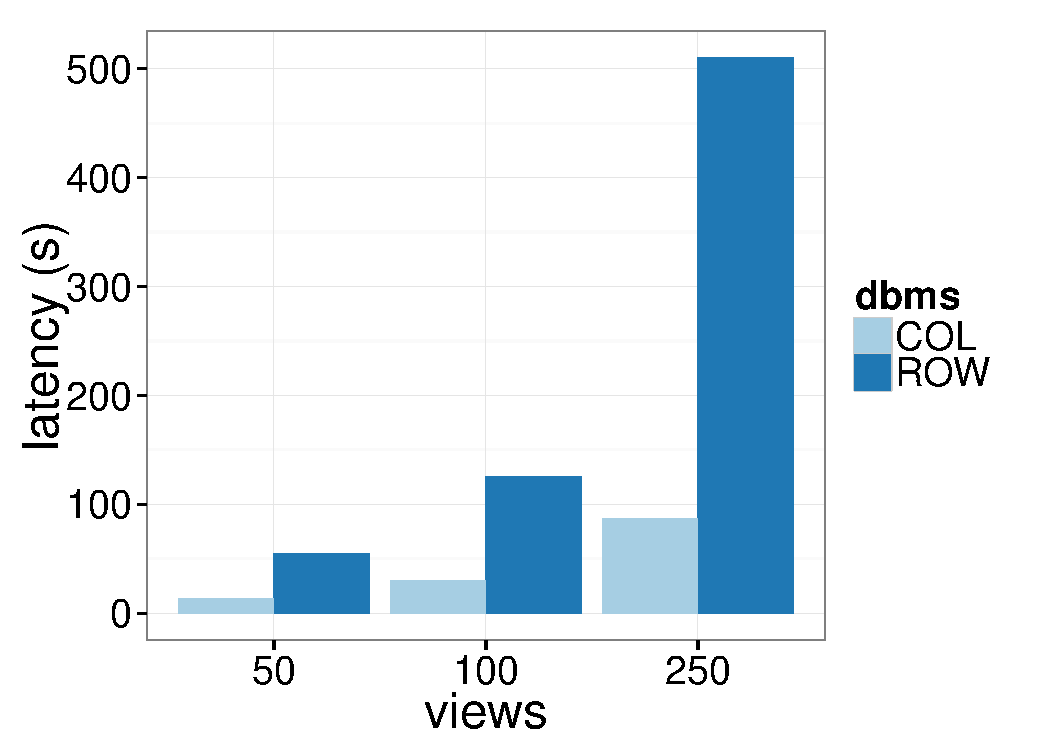
\includegraphics[width=4.2cm] {Images/baselines_by_views.pdf}}
% \caption{Latency vs. Num Views}
% \label{fig:baseline_views}
% \end{subfigure}
% \label{fig:baselines}
% \caption{Latency of Basic Framework}
% \end{figure}

\stitle{Combining Multiple Aggregates:} 
{\em \underline{Summary:} Combining view queries with the same group-by attribute
but different aggregates gives a 
3-4X speedup for both row and column stores.}
To study the limits of adding multiple aggregates to a single query, we ran \SeeDB
by varying the limit on the number of aggregates in any generated SQL query 
($n_{agg}$) between 1 and 20.
% We combine multiple view queries that have the same group-by (dimension) 
% attribute, but different aggregation (measure) attributes into one query.
% We ran these experiments on the SYN2 dataset 
% since it has a large number (20) of measure attributes.
% We varied the number of aggregate attributes 
% in a query between 1 and 20 (i.e., we grouped $n_{agg}$ view
% queries that share the same group-by attribute into one query
% that is issued to the DBMS).
The resulting latencies on the SYN dataset are shown in Figure \ref{fig:multi_agg} (log scale on the y-axis).
As we can see, latency reduces consistently with the number of aggregations performed 
per query.
The latency reduction is however not linear in $n_{agg}$ because
larger $n_{agg}$ values require maintenance of more state and access of more columns in a 
column store.
Overall, we get a 4X speedup for row stores and a 3X speed up for column stores.

\stitle{Parallel Query Execution:} 
{\em \underline{Summary:} Running view queries in parallel can offer significant
performance gains; however, there is an optimal number of parallel queries
beyond which performance degrades significantly.}
Executing \SeeDB-generated SQL queries in parallel can provide significant performance gains
because queries can share buffer pool pages.
However, a high degree of parallelism can degrade performance for a variety of reasons \cite{Postgres_wiki}. 
Figure \ref{fig:parallelism} illustrates this issue: we varied the maximum number of parallel queries
issued by \SeeDB and measured the resulting latency.
As expected, low levels of parallelism produced sizable performance gains but
high levels led to degraded performance.
For both row and column stores in our system, the optimal number of queries to 
run in parallel is approximately $16$ (equal to the number of cores). 
% This appears to hold true for both row or column stores. 
In general, we have found that choosing a degree of parallelism equal to the number of cores
% for these kinds of simple aggregation queries when data largely fits in memory,
is a reasonable rule of thumb. 
% \mpv{separate this from general study of parallel queries}

% \begin{figure}[h]
% \centering
% {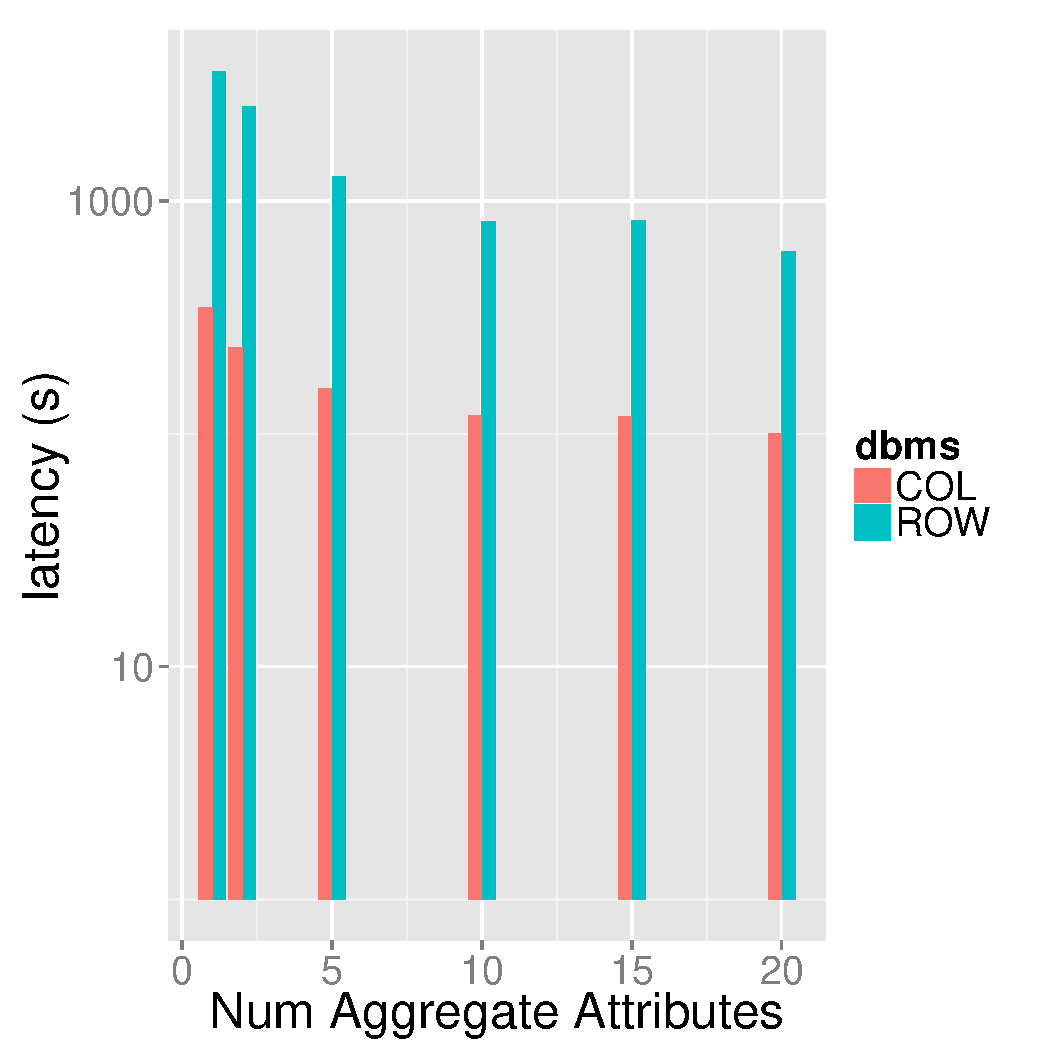
\includegraphics[width=6cm] {Images/multi_agg.pdf}}
% \caption{Latency vs. number of aggregates}
% \label{fig:multi_agg}
% \end{figure} 

\stitle{Combining Multiple Group-bys:} 
{\em \underline{Summary:} Combining multiple view queries with a single group-by attribute into a single query will multiple
grouping improves performance by 2.5X in row stores.}
We now study the effect of combining multiple queries each with a single group-by into one query.
Unlike the multiple aggregates optimization, the impact of combining group-bys
is unclear due to larger memory requirements as well as post-processing cost.
To verify our hypothesis that the ideal grouping must be one that keeps memory utilization
under a threshold, we ran an experiment with datasets SYN*-10 and SYN*-100 where
we varied the number of group-by attributes in \SeeDB-generated SQL queries ($n_{gb}$) 
between 1 and 10.
Since each attribute in SYN*-10 has 10 distinct values and that in SYN*-100
has 100, a query with $n_{gb}=p$ would require memory proportional to $\max(10^p,
num\_rows)$ for SYN*-10 and proportional to $\max(100^p, num\_rows)$ for SYN*-100.
The results of the experiment are shown in Figure \ref{fig:multi_gb_same}.
As the number of group-by attributes increases from 1 to 10, the latency of ROW (blue) decreases initially.
However, once the space budget (proxied by the number of distinct groups) exceeds 10000, latency increases significantly.
We see a similar trend for COL, but with a space budget of 100.\footnote{The different space
budgets can be explained based on the different internal parameteres and implementations of
the two systems.}
This empirically verified relation between memory usage and latency supports the use of 
our bin-packing optimization.

% We see that for the row-store, latency does improve (and then gets worse) as the
% number of group by attributes increases.  
% The best latency is obtained for 2 group by attributs in SYN3-100 and 4 attributes in SYN3-10.  
% This suggests that it is the number of distinct groups that matters most, since these 
% minima occur at 10,000 distinct groups in both cases (shown on \ref{fig:multi_gb_same} as the 
% two ``10000'' labels on the ROW lines).
% Beyond 5 attributes, the performance degrades drastically.  
%  For the column-store, we see a
% relatively small improvement in latency for 2 groups on SYN3-10, with 1 group being best for
% SYN3-100.  Here again it appears that the total number of groups (100 in the case of the column store) determines
% the overall optimal performance.
% After $10^5$ groups, the performance also becomes much worse for COL.

% In Section~\ref{sec:dbms_optimizations}, we described
%  how the impact of this optimization was not
% clear since it increases the total number of groups significantly and therefore
% leads to higher costs of processing intermediate results.
% To evaluate this optimization, we use the SYN3-10 and SYN3-100 datasets.
% We chose these datasets over SYN1 and SYN2 since we wanted to control
% the number of distinct groups in every attribute and consequently the number of
% distinct groups in every combination of attributes.
% In SYN3-10 for example, all dimensions have 10 distinct values and each
% dimension is independently generated. 
% Therefore, the total number of distinct
% groups produced by a query with $p$ group-by attributes is $\max(10^p,
% num\_rows)$.
% SYN3-100 similarly has 100 distinct values per attribute and produces
% $\max(10^p, num\_rows)$ groups for $p$ attributes.
% Our goal in these experiments is to determine if (a) combining multiple
% group-by attributes improved performance, and (b) whether it was the number of
% group-by attributes or the number of distinct groups produced by a query that
% predicted performance.

% We ran \SeeDB\ on SYN3-10 and SYN3-100, and varied the number of
% group-by attributes in view queries ($n_{gb}$) between 1 and 10.


% These results show that 1) combining group by attributes can improve performance, up to a point, and 2) the optimal
% number of attributes is determined by the total number of distinct groups that will result.  Different systems have a different
% number of optimal groups, and this number is somewhat implementation dependent.  The performance degradation with
% large numbers groups likely result from cache misses or other (non)-locality effects
% as the memory required for the grouping grows, or as the system switches to external algorithms for these
% operations.

% \begin{figure}[h]
% \centering
% \begin{subfigure}{0.49\linewidth}
% \centering
% {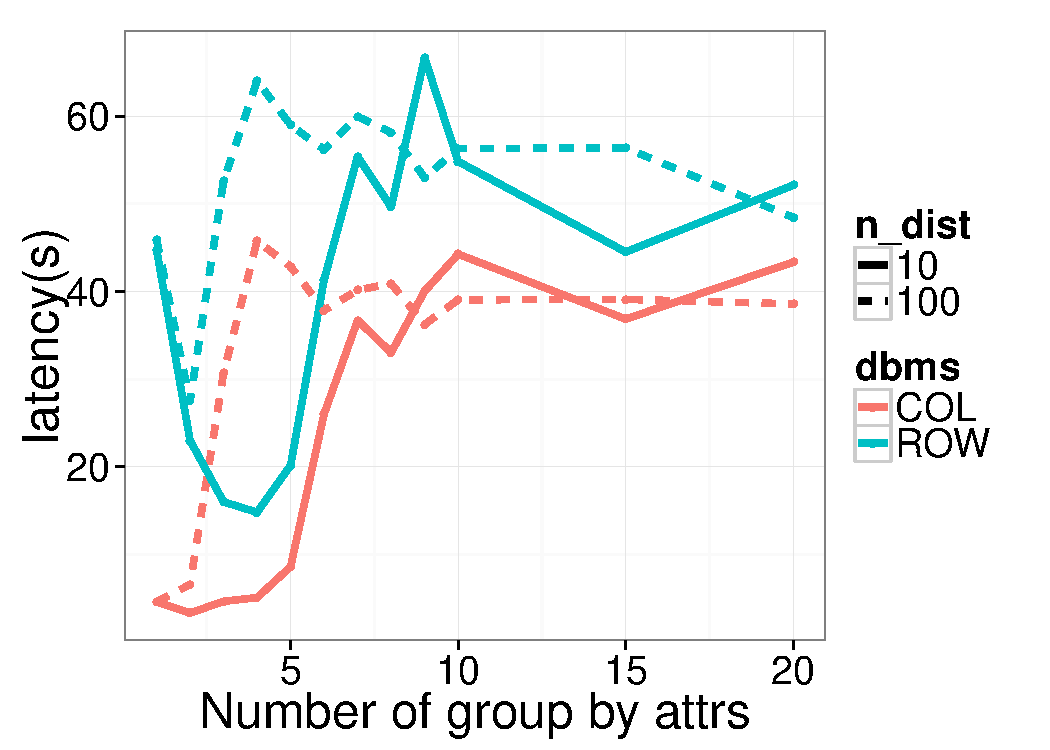
\includegraphics[width=4.2cm] {Images/multi_gb_same.pdf}}
% \caption{Latency vs. Num of Groups}
% \label{fig:multi_gb_same}
% \end{subfigure}
% \begin{subfigure}{0.49\linewidth}
% \centering
% {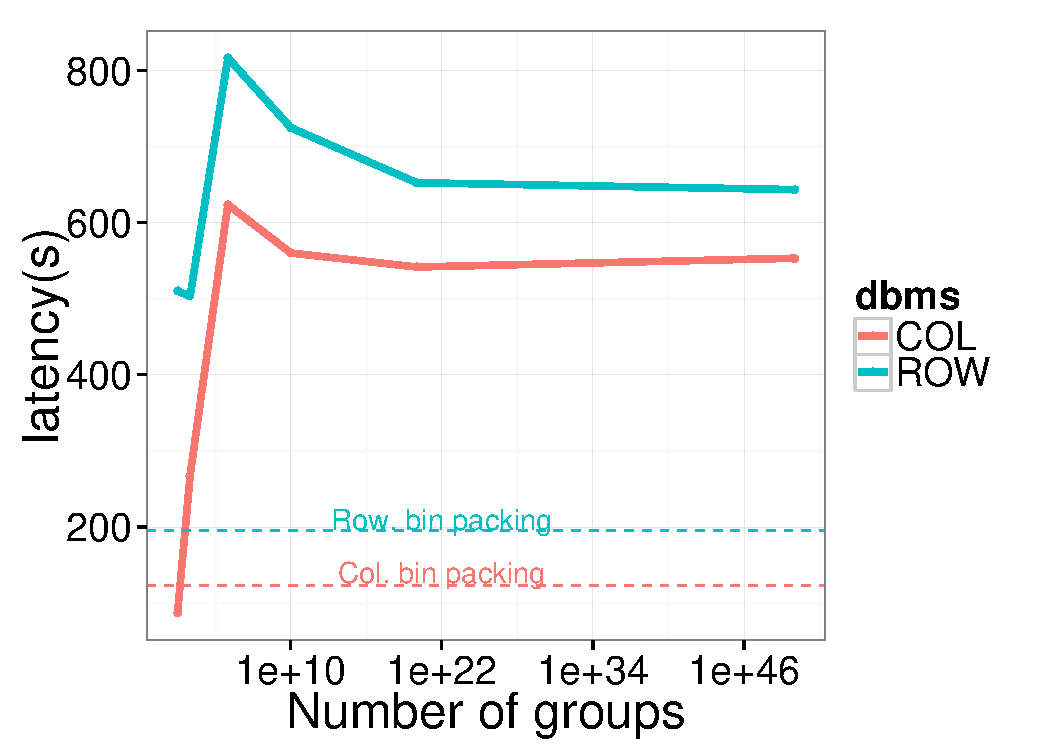
\includegraphics[width=4.2cm] {Images/multi_gb.pdf}}
% \caption{Latency vs. Num Dimensions}
% \label{fig:multi_gb_bp}
% \end{subfigure}
% \label{fig:multi_gb}
% \caption{Effect of combining multiple groups}
% \end{figure}

% We can guard against the above performance degradation by ensuring that the
% number of distinct groups never goes beyond a pre-configured upper limit.
% From Figure \ref{fig:multi_gb_same}, we see that this limit is approximately
% $10^4$ for the row-store and $10^2$ for the column store.

Next, we use the space constraint derived in the previous experiment
to perform optimal grouping via bin-packing (Section \ref{subsec:mult_gb}).
% With knowledge of this upper limit on the number of distinct groups, we can now
% apply our grouping technique based on bin packing (Section \ref{subsec:mult_gb}) to optimally
% group the dimension attributes.
% Bin-packing ensures that the number of distinct groups produced by any query is
% less than $10^4$ (for rows) or $10^2$ (for columns).
Figure \ref{fig:multi_gb_bp} shows the results of multi-attribute group-bys on SYN where
$n_{gb}$ was varied between 1 and 20 (solid lines).
Note that SYN contains attributes with variable number of distinct values (between 1 and 1000). 
Therefore, a query with
$n_{gb}$=3 can have memory utilization anywhere from 1 unit to $10^9$ units, thus breaking the
memory threshold.
Since the latency results in this experiment are greatly impacted by how attributes are grouped,
we randomize the grouping 20 times and report average latency.
The dotted lines show the latency obtained by performing optimal grouping via bin-packing.
We observe a significant, 2.5X improvement in ROW latency due to bin-packing.
This can be attributed to the fact that ROW's large threshold on space (10000) allows many queries
to be combined.
COL, on the other hand, shows a much less pronounced speedup. This is expected since its memory
threshold of 100 biases the optimal grouping to contain many single attribute groupings.
% To obtain these metrics, we randomly grouped attributes into groups of size $n_{gb}$ and ran
% the experiment 20 times to get average latency.
% We also show the performance of \SeeDB\ when we use bin-packing to optimally group the dimension
% attributes.
% As seen in the chart, grouping based on bin-packing is always superior to grouping based
% on the number of attributes $n_{gb}$. 
% In fact, for the row-store, bin-packing reduces latency by a factor of 2.5X. 
% Although benefit is less pronounced, it is also noticeable for column-stores.


% of bin packing when the number of groups is set to $10^2$ (columns) or $10^4$ (rows) (dotted lines).
% In the former strategy, we randomly group attributes into groups of size
% $n_{gb}$. 
% Since the latency for this strategy will depend on the particular grouping of
% attributes, we repeated this experiment 20 times and report the average latency.
% As we can see from the chart, bin-packing is always superior to grouping
% based on attribute number, given the optimal bin-size for a particular system.
% We see that for the row-store, bin-packing reduces latency by a factor of 2.5X. 
% Although benefit is less pronounced, it is still noticeable for column-stores.
 
%For other systems, we recommend users that they set the number of parallel
%queries to the maximum number of parallel queries that can be run in
%their DBMS without performance degradation.
%If this number is not easily available, a simple experiment as shown in Figure
%\ref{fig:parallelism} can help approximate the right amount of parallelism. \\

% \noindent {\it Combining Target and Comparison Views}:
% The last optimization we evaluate is that of combining the target and comparison
% views and running a single SQL query per view as opposed to two.
% We expected this optimization to roughly halve the latency since each query
% takes one table scan instead of two.\\

\begin{figure}[h]
	\centering
	\begin{subfigure}{0.48\linewidth}
		\centering
		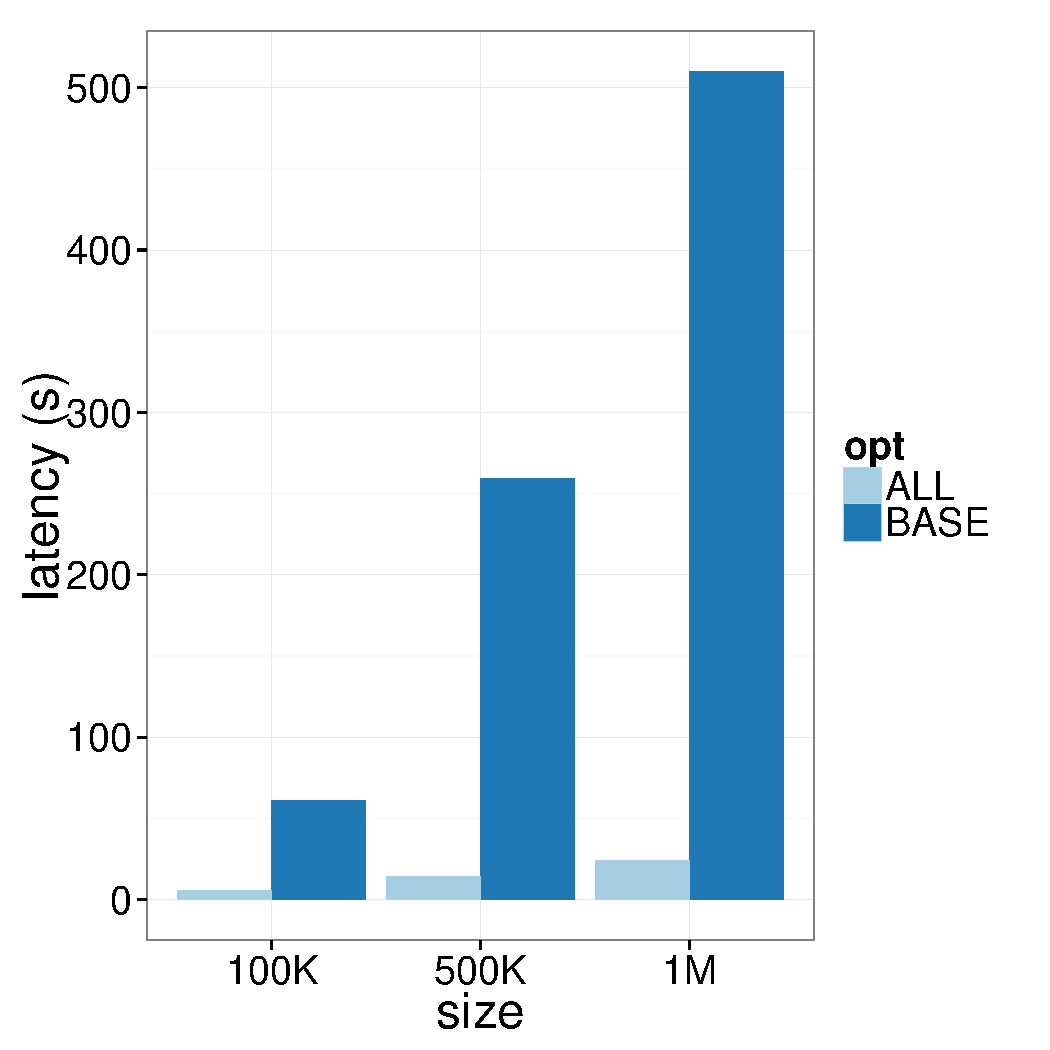
\includegraphics[width=4.4cm] {Images/row_all_none_by_size.pdf}
		\caption{Row store latencies by size}
		\label{fig:row_all_none_size}
	\end{subfigure}
	% \begin{subfigure}{0.24\linewidth}
	% 	\centering
	% 	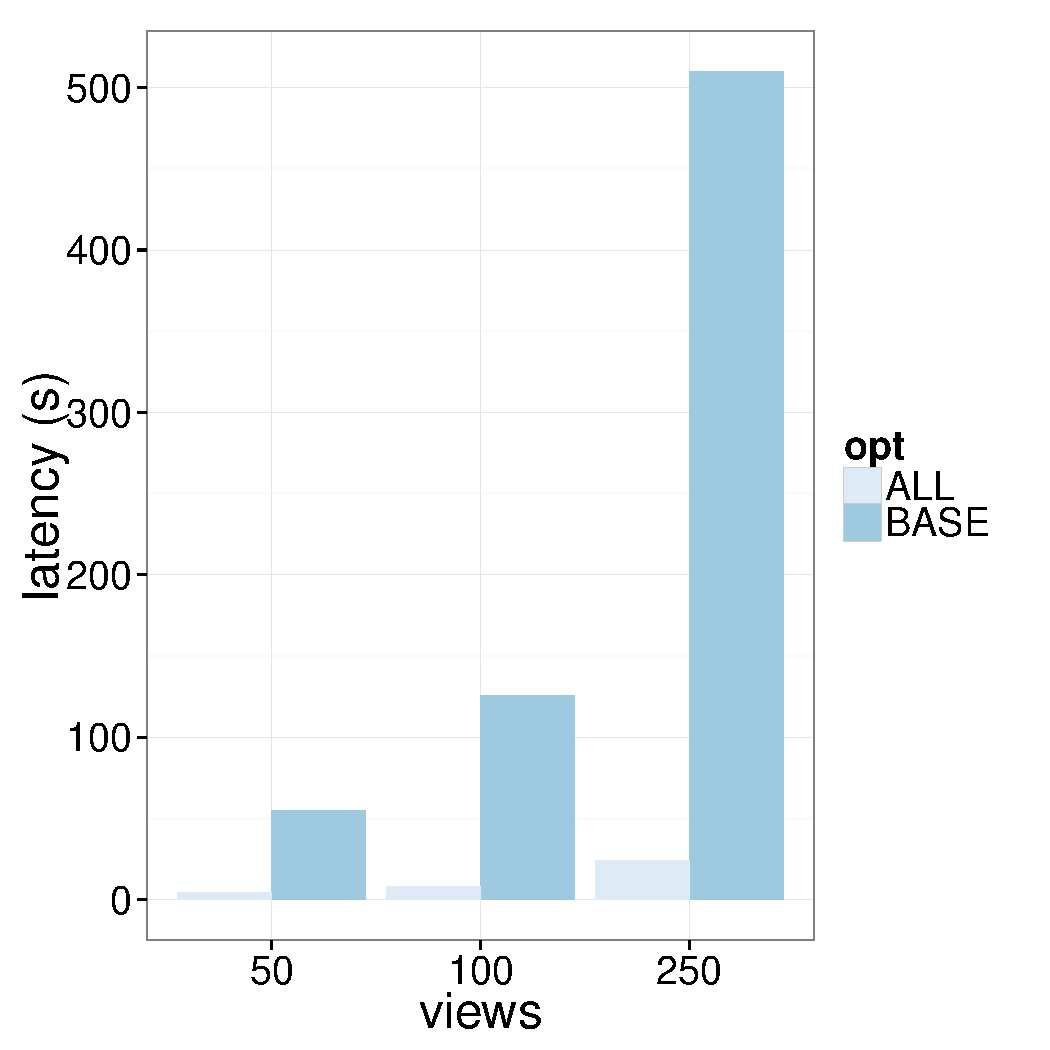
\includegraphics[width=4.6cm] {Images/row_all_none_by_views.pdf}
	% 	\caption{Row store latencies by views}
	% 	\label{fig:row_all_none_views}
	% \end{subfigure}
	% \begin{subfigure}{0.24\linewidth}
	% 	\centering
	% 	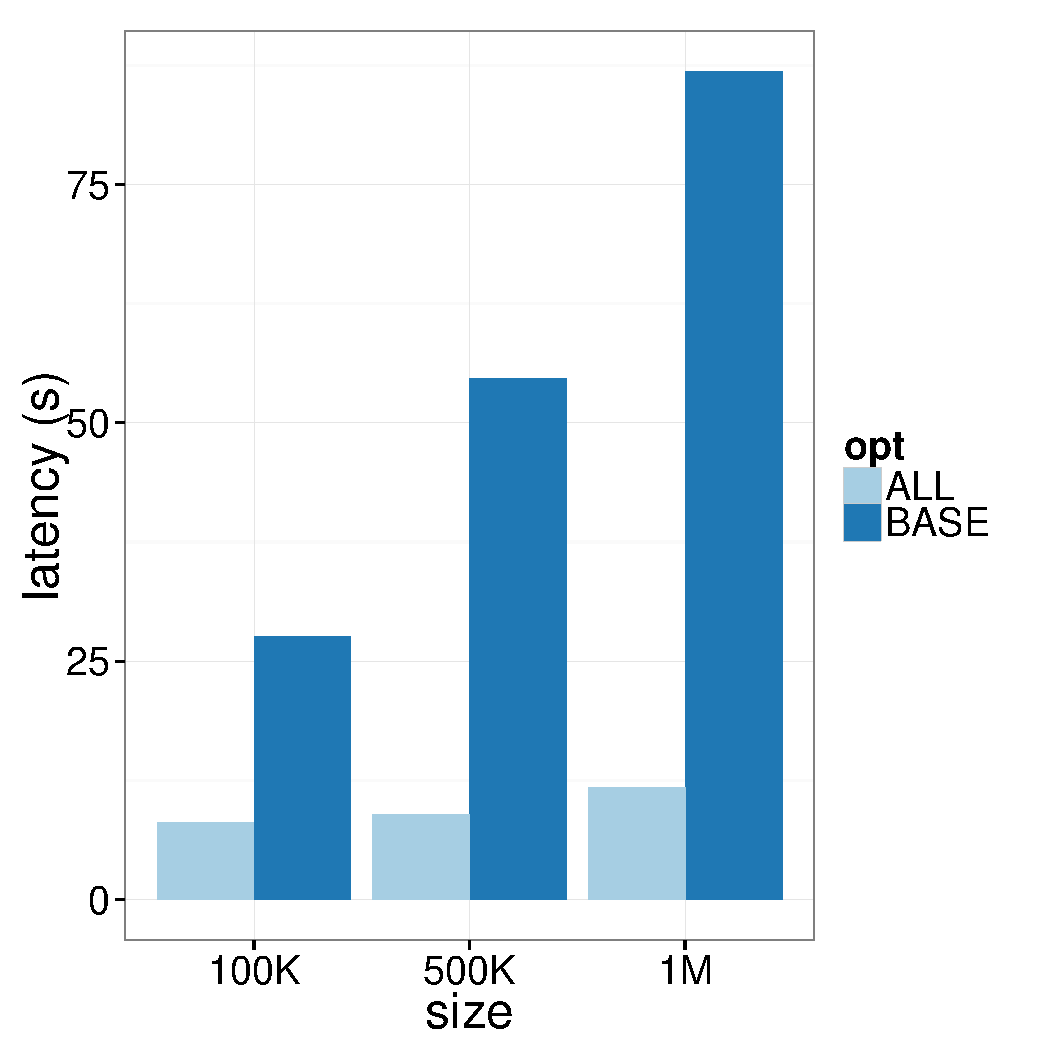
\includegraphics[width=4.6cm] {Images/col_all_none_by_size.pdf}
	% 	\caption{Column store latencies by size}
	% 	\label{fig:col_all_none_size}
	% \end{subfigure}
	\begin{subfigure}{0.48\linewidth}
		\centering
		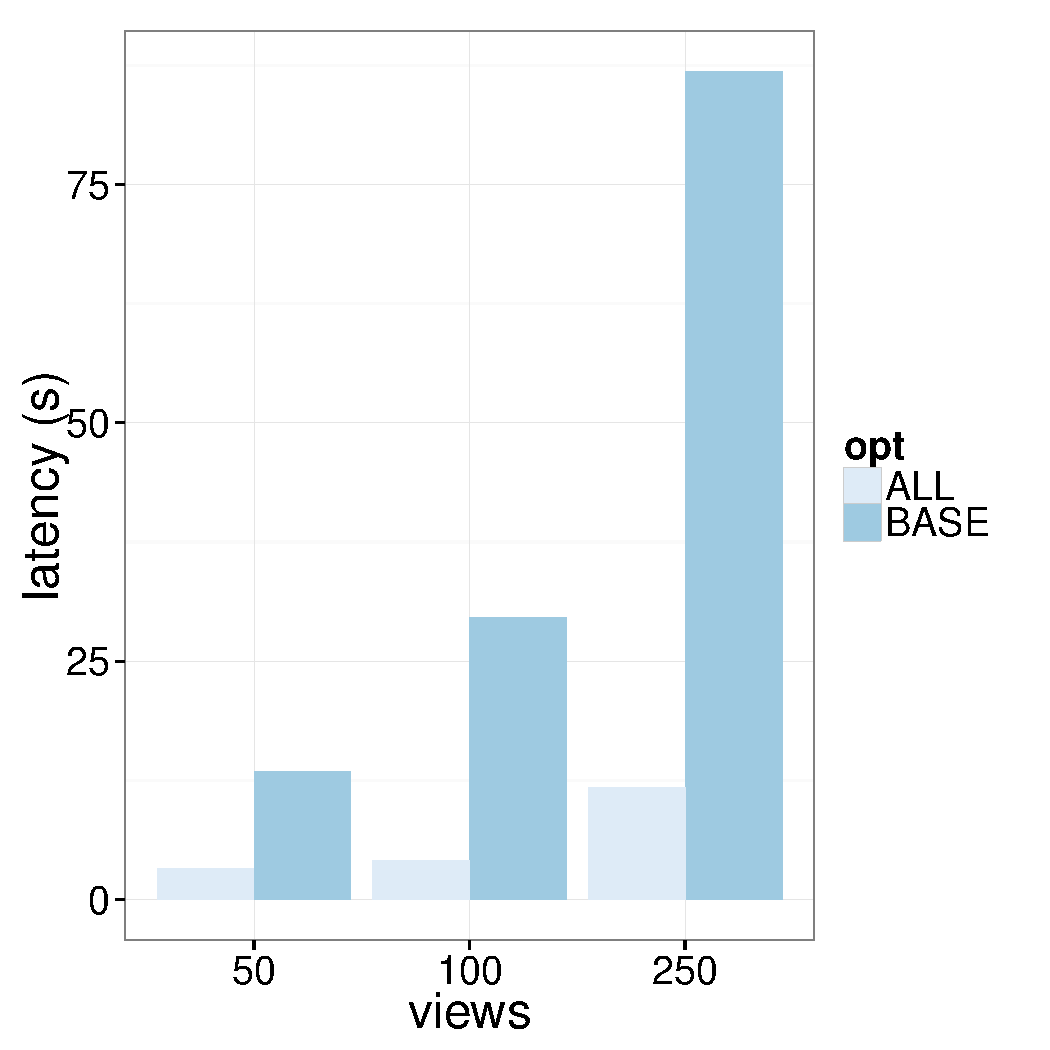
\includegraphics[width=4.4cm] {Images/col_all_none_by_views.pdf}
		\caption{Column store latencies by views}
		\label{fig:col_all_none_views}
	\end{subfigure}
	\vspace{-10pt}
	\caption{Effect of All Optimizations}
	\label{fig:all_opt}
	\vspace{-15pt}
\end{figure}


\stitle{All Sharing Optimizations:} 
{\em \underline{Summary:} Applying all of our sharing optimizations
leads to a speedup of up to 20X for row stores, and 8X for column stores;
column stores are still much faster than row stores.}
Based on the optimal parameters identified from the previous experiments, we combined 
our optimizations to obtain the best performance. 
% Now that we have explored the proposed optimizations in detail, we pick the optimal
% parameters discovered above and combine our optimizations to get the maximum
% performance gain. 
For the row store, we applied all the above optimizations with $n_{agg}$ set to
the total number of measure attributes, maximum number of group-bys set to $10^4$ and
parallelism set to $16$.
For the column store, we set $n_{agg}$ and number of parallel queries similarly
but did not apply the group-by optimization. 
Figure~\ref{fig:all_opt} shows the latency of \SeeDB\ on SYN when all
optimizations have been applied.
We see that our optimizations lead to a speed up of 20X for ROW 
(Figures~\ref{fig:all_opt}a) and a speedup of 10X in COL (Figures~\ref{fig:all_opt}b).
Furthermore, we notice that our optimizations are most effective for datasets with 
large sizes and many views. This is particularly true for ROW where each scan
of a large table is expensive, and hence reduction in number of queries 
has larger benefits.
% , with proportionally larger speedups as these numbers grow.

\techreport{
\stitle{Resource Utilization:}
Finally, we examine the resource utilization for the DBMS-backed engine.
With the DBMS-backed execution engine, each \SeeDB query translates into 50+ optimized SQL queries.
We call this 50X increase in queries as {\it query bloat}. 
Each SQL query scans the same data and stores individual state such as iterators, counters, buffers etc.
In addition, we find that although parallel queries share buffer pool pages, running a large number of view queries in
parallel can lead to thrashing due to timing issues.
As a result, we find the DBMS-backed engine has large overheads of memory, CPU and query state due to the query bloat.}

% In summary, the above set of experiments shows that the application of well-designed optimizations
% and parallelism can reduce \SeeDB\ latency by 8-20X depending on the DBMS.
% We notice, however, that in spite of aggressive optimizations, the latencies with sharing optimizations are between 10-20s.
% Such latencies are unacceptable in any interactive system.
% Moreover, we observe that query bloat associated with each \SeeDB invocation unnecessarily consumes DBMS resources.
% In an environment where the DBMS serves multiple users with more than just visualization
% software, this approach is clearly wasteful. 
% As a result, we see need for a solution that can provide much lower latencies 
% and have a smaller resource footprint.
% In the next section, we evaluate the performance of our custom execution engine that promises these advantages.